%!TEX root = ../paper.tex
\chapter{环境配置}
	\section{CMake}
		\subsection{简介}
			\par CMake是个开源的跨平台自动化建构系统,它用配置文件控制建构过程(build process)的方式和Unix的Make相似,只是CMake的配置文件取名为CMakeLists.txt。Cmake先产生标准的建构档(如Unix的Makefile或Windows Visual C++的projects/workspaces),然后再依一般的建构方式使用。这使得熟悉某个集成开发环境(IDE)的开发者可以用标准的方式建构他的软件。CMake可以编译源代码、制做程序库、产生适配器(wrapper)、还可以用任意的顺序建构可执行文件,支持二进档和源代码在同一个目录树中建构和二进档在别的目录里建构,因此以很容易从同一个源代码目录树中建构出多个二进档。CMake也支持静态与动态程序库的建构\ucite{ wiki:CMake}。
			\par GNU Radio采用CMake构建,所以简单介绍一下CMake的使用方法,方便后续开发者理解GNU Radio模块的编写以及在此基础上构建自己的应用。
			\par CMake的源码已托管至GitHub(\href{https://github.com/Kitware/CMake.git}{https://github.com/Kitware/CMake.git})。
		\subsection{安装}
			\label{sec:CMake}
			\par 在Ubuntu环境下可以直接执行\lstinline[language=sh]{sudo apt install cmake}来安装。也能使用源码来编译CMake。
			\begin{lstlisting}[ language= sh ]
git clone https://github.com/Kitware/CMake.git
./bootstrap && make && make install
			\end{lstlisting}
			\par 在Windows下可以在CMake官网(\href{https://cmake.org/download/}{https://cmake.org/download/})选择与自己系统版本相对应的版本进行安装。如果使用Visual Studio 2015及以上版本,可以直接用Visual Studio打开项目目录,会自动使用CMake构建相应的解决方案。
		\subsection{构建CMake项目}
			\par CMake要求每个目录下均有一个\lstinline{CMakeLists.txt}文件,一个常见的CMake项目的目录结构如下:
			\dirtree{%
				.1 ..
				.2 app.
				.3 CMakeLists.txt.
				.3 main.cc.
				.3 main.h.
				.2 include.
				.3 CMakeLists.txt.
				.3 test.h.
				.2 lib.
				.3 test\_impl.cc.
				.3 test\_impl.h.
				.2 CMakeLists.txt.
				.2 README.md.
			}
			\par 其中:
			\par \lstinline{app}目录下放置\lstinline{main}函数所在文件,可以同时包含多个将要生成的程序,最终将在\lstinline{./build/app/}目录下生成与该文件同名的可执行文件,在\lstinline{./build/app/}目录下执行\lstinline{./main}即可运行。
			\par \lstinline{include}目录下放置项目所需要的头文件。
			\par \lstinline{lib}目录下为该项目生成的库文件。
			\par \lstinline{README.md}为用Markdown格式书写的说明文档。
			\par 顶层目录下的\lstinline{CMakeLists.txt}内容如下:
			\begin{lstlisting}
project(main)
cmake_minium_required(VERSION 2.6)
aux_source_directories(. DIR_SRC)
include_directories(include)
add_executable(main ${DIR_SRC})
add_subdirectory(lib)
target_link_libraries(main test)
			\end{lstlisting}
			\par \lstinline{/lib/CMakeLists.txt}内容如下:
			\begin{lstlisting}
aux_source_directories(. DIR_TEST_DIR)
add_library(test ${DIR_TEST_DIR})
# add_library(test STATIC ${DIR_TEST_DIR})
			\end{lstlisting}
			\par \lstinline{/include/CMakeLists.txt}文件可以为空,有公共库可以用\lstinline[language=sh]{install(file name)}来安装进系统环境。
			\par 编译运行
			\begin{lstlisting}[ language = sh ]
mkdir build
cd build
cmake ..
make
			\end{lstlisting}
			\par 便会在\lstinline{/build/build/app}目录下生成相应的可执行文件。在使用git时进行版本控制注意在gitignore中添加build目录,以免git对编译后产生的文件进行跟踪,以免编译一次产生一次更改,造成版本库的混乱。有众多的开源项目基于CMake构建,使用这些程序时编译完成以后还需要使用以下命令来将其置入系统路径,使其能够在命令行下直接执行。
			\begin{lstlisting}
sudo make install
			\end{lstlisting}
			\par 如果编译的动态库还需要将其链接:
			\begin{lstlisting}[ language= sh ]
sudo ldconfig
			\end{lstlisting}
	\section{Boost C++ Libraries}
		\subsection{简介}
			\par Boost C++ 库(Libraries)是一组扩充C++功能的经过同行评审(Peer-reviewed)且开放源代码程序库。大多数的函数为了能够以开放源代码、封闭项目的方式运作,而授权于Boost软件许可协议(Boost Software License)之下。许多Boost的开发人员是来自C++标准委员会,而部分的Boost库成为C++的TR1标准之一\ucite{ wiki:Boost}。
			\par GNU Radio与gr-dvbt中调用了Boost库中的众多函数,需要安装该库才能够进行编译,执行以下命令进行安装。
			\begin{lstlisting}[ language= sh ]
sudo apt install libboost-all-dev
			\end{lstlisting}
			\par Boost的源码已托管于GitHub(\href{https://github.com/boostorg}{https://github.com/boostorg})。
	\section{Doxygen}
		\subsection{简介}
			\par Doxygen是一个C++、C、Java、Objective-C、Python、IDL(CORBA和Microsoft flavors)、Fortran、VHDL、PHP、C\#和D语言的文档生成器。可以在大多数类Unix以及Mac OS X和Microsoft Windows上运行。Doxygen文档是直接写在源代码中,因此比较容易保持更新。Doxygen支持交叉引用文档和源代码,使文件的读者可以很容易地引用实际的源代码\ucite{ wiki:Doxygen}。
			\par GNU Radio的API文档(\href{https://gnuradio.org/doc/doxygen/index.html}{https://gnuradio.org/doc/doxygen/index.html})由Doxygen生成。
			\par 在编写程序的过程中使用符合Doxygen规范的注释块,如有需要,构建时可以使用Doxygen生成如图\ref{fig:doxygen_gnuradio}的说明文档以及如图\ref{fig:doxygen_dvbt_map}调用关系图。
			\begin{figure}[htbp]
				\centering
				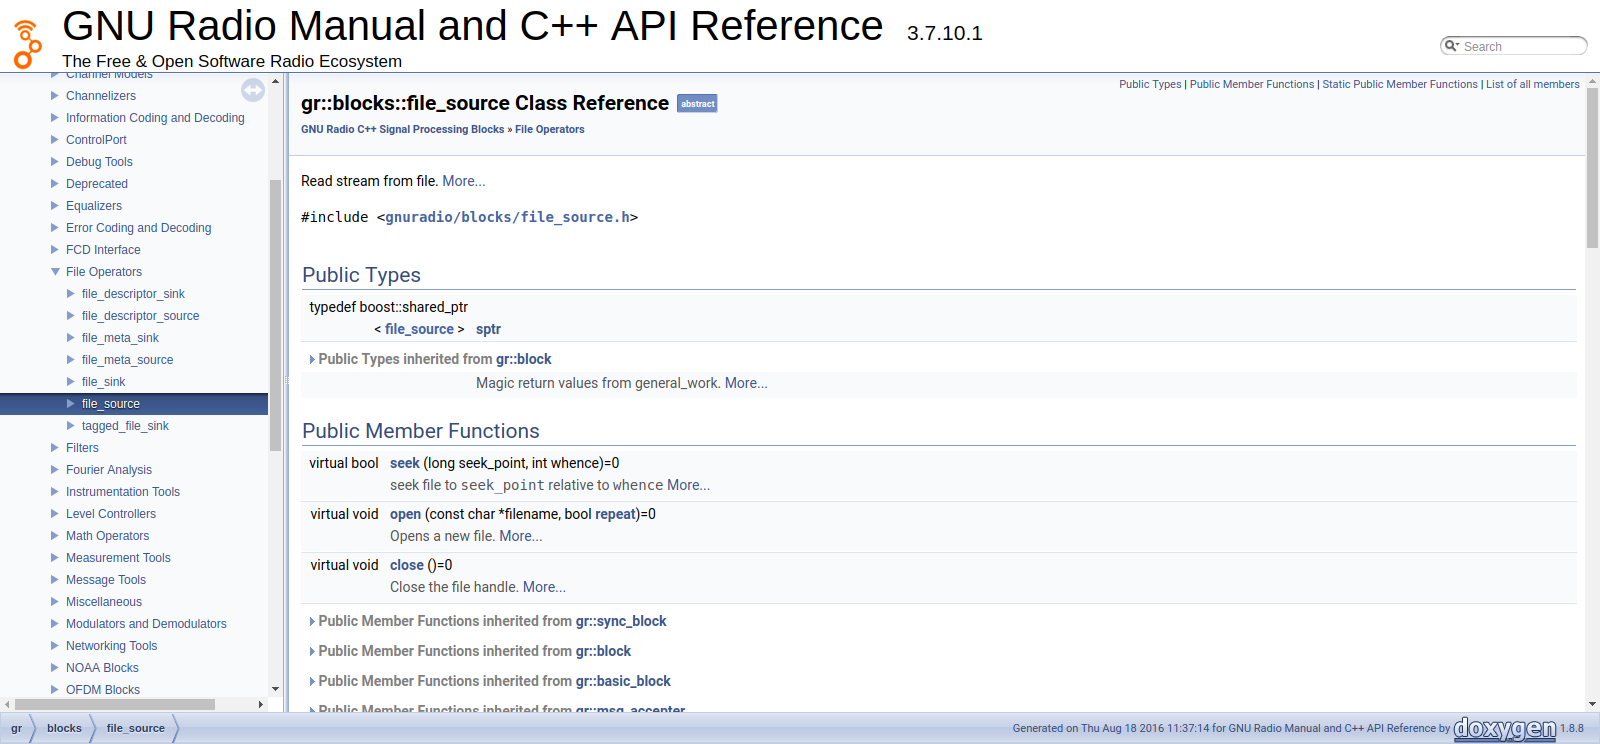
\includegraphics[width=13cm]{figures/doxygen_gnuradio.png}
				\caption{Doxygen生成的GNU Radio说明文档}
				\label{fig:doxygen_gnuradio}
			\end{figure}
			\begin{figure}[htbp]
				\centering
				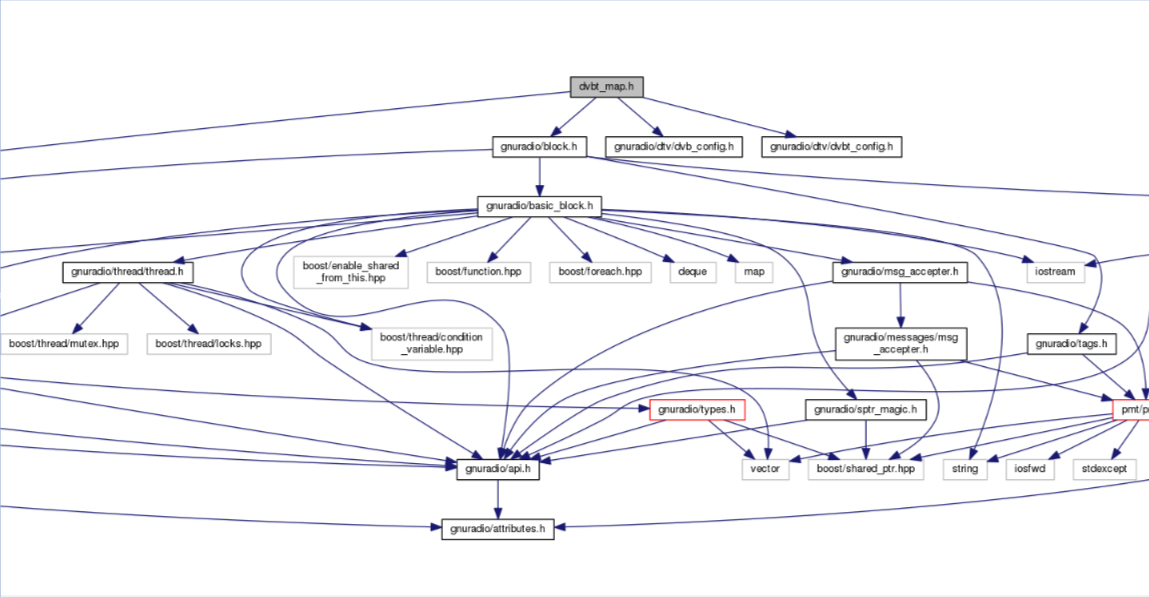
\includegraphics[width=13cm]{figures/doxygen_dvbt_map.png}
				\caption{Doxygen生成的调用关系图}
				\label{fig:doxygen_dvbt_map}
			\end{figure}
			\par Doxygen的源码已托管于GitHub(\href{https://github.com/doxygen/doxygen}{https://github.com/doxygen/doxygen})。
		\subsection{使用方法}
			\par 在文件中使用Doxygen规范的注释\ucite{ wiki:Doxygen}。
			\par 一般文件:
			\begin{lstlisting}
/**
* <A short one line description>
*
* <Longer description>
* <May span multiple lines or paragraphs as needed>
*
* @param  Description of method's or function's input parameter
* @param  ...
* @return Description of the return value
*/
			\end{lstlisting}
			\par 头文件:
			\begin{lstlisting}
/*!
* <A short one line description>
*
* <Longer description>
* <May span multiple lines or paragraphs as needed>
*
* @param  Description of method's or function's input parameter
* @param  ...
* @return Description of the return value
*/
			\end{lstlisting}
			\par 在工程目录下执行\lstinline[language=sh]{doxygen -g}生成Doxyfile,修改\lstinline{OUTPUT_DIRECTORY}为自己想要的生成目录与其他参数,最后执行\lstinline{doxygen Doxyfile}即可生成\lstinline{latex}和\lstinline{html}目录,打开\lstinline{html}目录下的\lstinline{index.html}即可看到生成的网页格式的说明文档以及文件间的调用关系图,在\lstinline{latex}目录下运行\lstinline{./make}还可以生成pdf文件。
			\par Doxygen还能嵌入到CMake中,在\lstinline{CMakeLists.txt}中添加以下命令
			\begin{lstlisting}
# add a target to generate API documentation with Doxygen

FIND_PACKAGE(Doxygen)
OPTION(BUILD_DOCUMENTATION "Create and install the HTML based API documentation (requires Doxygen)" ${DOXYGEN_FOUND})

IF(BUILD_DOCUMENTATION)
	IF(NOT DOXYGEN_FOUND)
		MESSAGE(FATAL_ERROR "Doxygen is needed to build the documentation.")
	ENDIF()

	SET(doxyfile_in ${CMAKE_CURRENT_SOURCE_DIR}/Doxyfile.in)
	SET(doxyfile ${CMAKE_CURRENT_BINARY_DIR}/Doxyfile)

	CONFIGURE_FILE(${doxyfile_in} ${doxyfile} @ONLY)

	ADD_CUSTOM_TARGET(doc
		COMMAND ${DOXYGEN_EXECUTABLE} ${doxyfile}
		WORKING_DIRECTORY ${CMAKE_CURRENT_BINARY_DIR}
		COMMENT "Generating API documentation with Doxygen"
		VERBATIM)

	INSTALL(DIRECTORY ${CMAKE_CURRENT_BINARY_DIR}/html DESTINATION share/doc)
ENDIF()
			\end{lstlisting}
			\par 使用CMake生成\lstinline{makefile}以后,可以使用\lstinline{make doc}来生成API文档。
	\section{Python}
		\subsection{简介}
			\par Python,是一种面向对象、解释型的计算机程序语言。它包含了一组功能完备的标准库,能够轻松完成很多常见的任务。它的语法简单,与其它大多数程序设计语言使用大括号不一样,它使用缩进来定义语句块,经常被当作脚本语言用于处理系统管理任务和网络程序编写,然而它也非常适合完成各种高级任务。Python支持命令式程序设计、面向对象程序设计、函数式编程、面向侧面的程序设计、泛型编程多种编程范式\ucite{ wiki:Python}。
			\par Python简单的语法能够让开发者专注于算法,而不用去纠结语法上的问题,其众多的第三方库也给开发者带来了极大的便利,诸如用于科学计算的NumPy库已经能够替代Matlab的一些功能,所以Python语言具有很高的开发效率,已经被广泛地应用于机器学习、科学计算、Web后端、数字图像处理等众多领域。可以预见,在不久的将来也会在数字信号处理与通信工程领域大放异彩。
			\par GNU Radio采用Python来连接各个模块,在模块间传递参数,支持直接Python编程,但是由于Python执行效率较低,所以底层采用C++来提高性能,通过SWIG将C++类跟函数封装为Python中的模块,实现了性能与效率的综合。
			\par 一个不错的Python学习网站是廖雪峰的官方网站(\href{http://www.liaoxuefeng.com/}{http://www.liaoxuefeng.com/}),此处不再赘述。
			\par Python源码可以从\href{https://www.python.org/downloads/source/}{https://www.python.org/downloads/source/}下载。
	\section{SWIG}
		\subsection{简介}
			\par SWIG是个帮助使用C或者C++编写的软件能与其它各种高级编程语言进行嵌入联接的开发工具。SWIG能应用于各种不同类型的语言包括常用脚本编译语言例如Perl, PHP, Python, Tcl, Ruby and PHP。SWIG普遍应用于创建高级语言解析或汇编程序环境,用户接口,作为一种用来测试C/C++或进行原型设计的工具\ucite{ wiki:SWIG}。
			\par GNU Radio使用C++编写底层函数以实现性能最大化,使用SWIG将其中公有函数封装为Python的模块,极大的方便了开发者直接使用Python作为开发语言。GNU Radio的SWIG文件为\lstinline[language=sh]{swig}目录下的\lstinline[language=sh]{*.i}文件。
			\par SWIG的源码已托管于GitHub(\href{https://github.com/swig/swig}{https://github.com/swig/swig})。
			% TODO:用法
	\section{USRP}
		\subsection{简介}
			\par 通用软件无线电外设(USRP)是由Ettus Research及其母公司National Instruments设计和销售的一系列软件定义无线电设备。由Matt Ettus领导的团队开发,USRP产品系列旨在成为软件无线电相对便宜的硬件平台,已经被研究实验室,大学和业余爱好者广泛使用。大多数USRP通过高速链路连接到主机,主机软件用于控制USRP硬件和发送/接收数据,一些USRP模型还将主机的一般功能与嵌入式处理器集成,从而允许USRP设备以独立的方式运行。USRP系列设计之初便有很高的可修改性,许多产品是开源硬件,所有USRP型号的电路板原理图均可免费下载,所有USRP产品均采用开源的UHD驱动程序进行控制。USRP通常与GNU Radio软件套件一起使用,以创建复杂的软件定义无线电系统\ucite{ wiki:USRP}。
			\begin{figure}[htbp]
				\centering
				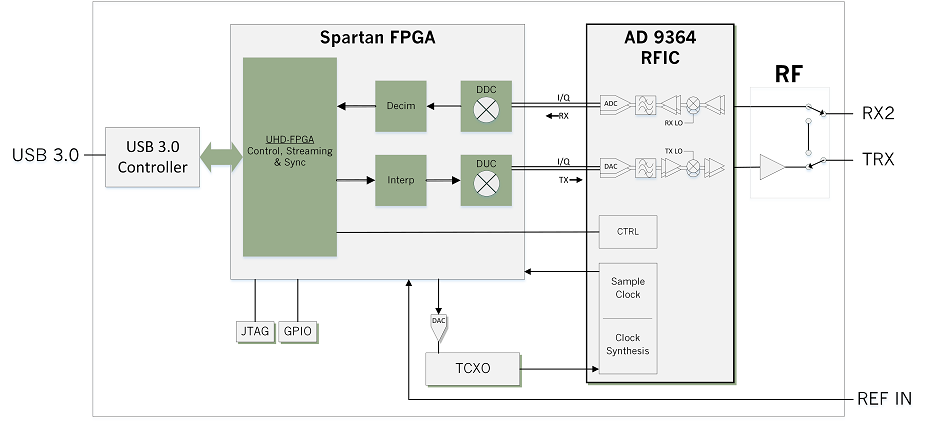
\includegraphics[width=13cm]{figures/USRP_B200mini_BD.png}
				\caption{USRP\_B200mini\_原理图}
				\label{fig:USRP_B200mini_原理图}
			\end{figure}
			\par UHD的源码已托管于GitHub(\href{https://github.com/EttusResearch/uhd}{https://github.com/EttusResearch/uhd})。
		\subsection{UHD}
			\par UHD是适用于USRP相关设备的开源的驱动程序,安装完成GNU Radio以后会自动安装UHD相关软件,USRP B200 mini需要UHD3.9.0及以上版本,使用版本过低会导致USRP无法识别。UHD提供了一些简单信号发生函数,能够用来实现一些简单的测试。
			\par 首次使用需要执行
			\begin{lstlisting}[ language = sh ]
uhd_images_downloader
			\end{lstlisting}
			\par 来下载USRP需要的镜像,以便之后的使用。
			\par 执行
			\begin{lstlisting}[ language = sh ]
uhd_siggen -f 900000000
			\end{lstlisting}
			\par 来产生一个如图\ref{fig:uhd_siggen}的正弦波。
			\begin{figure}[htp]
				\centering
				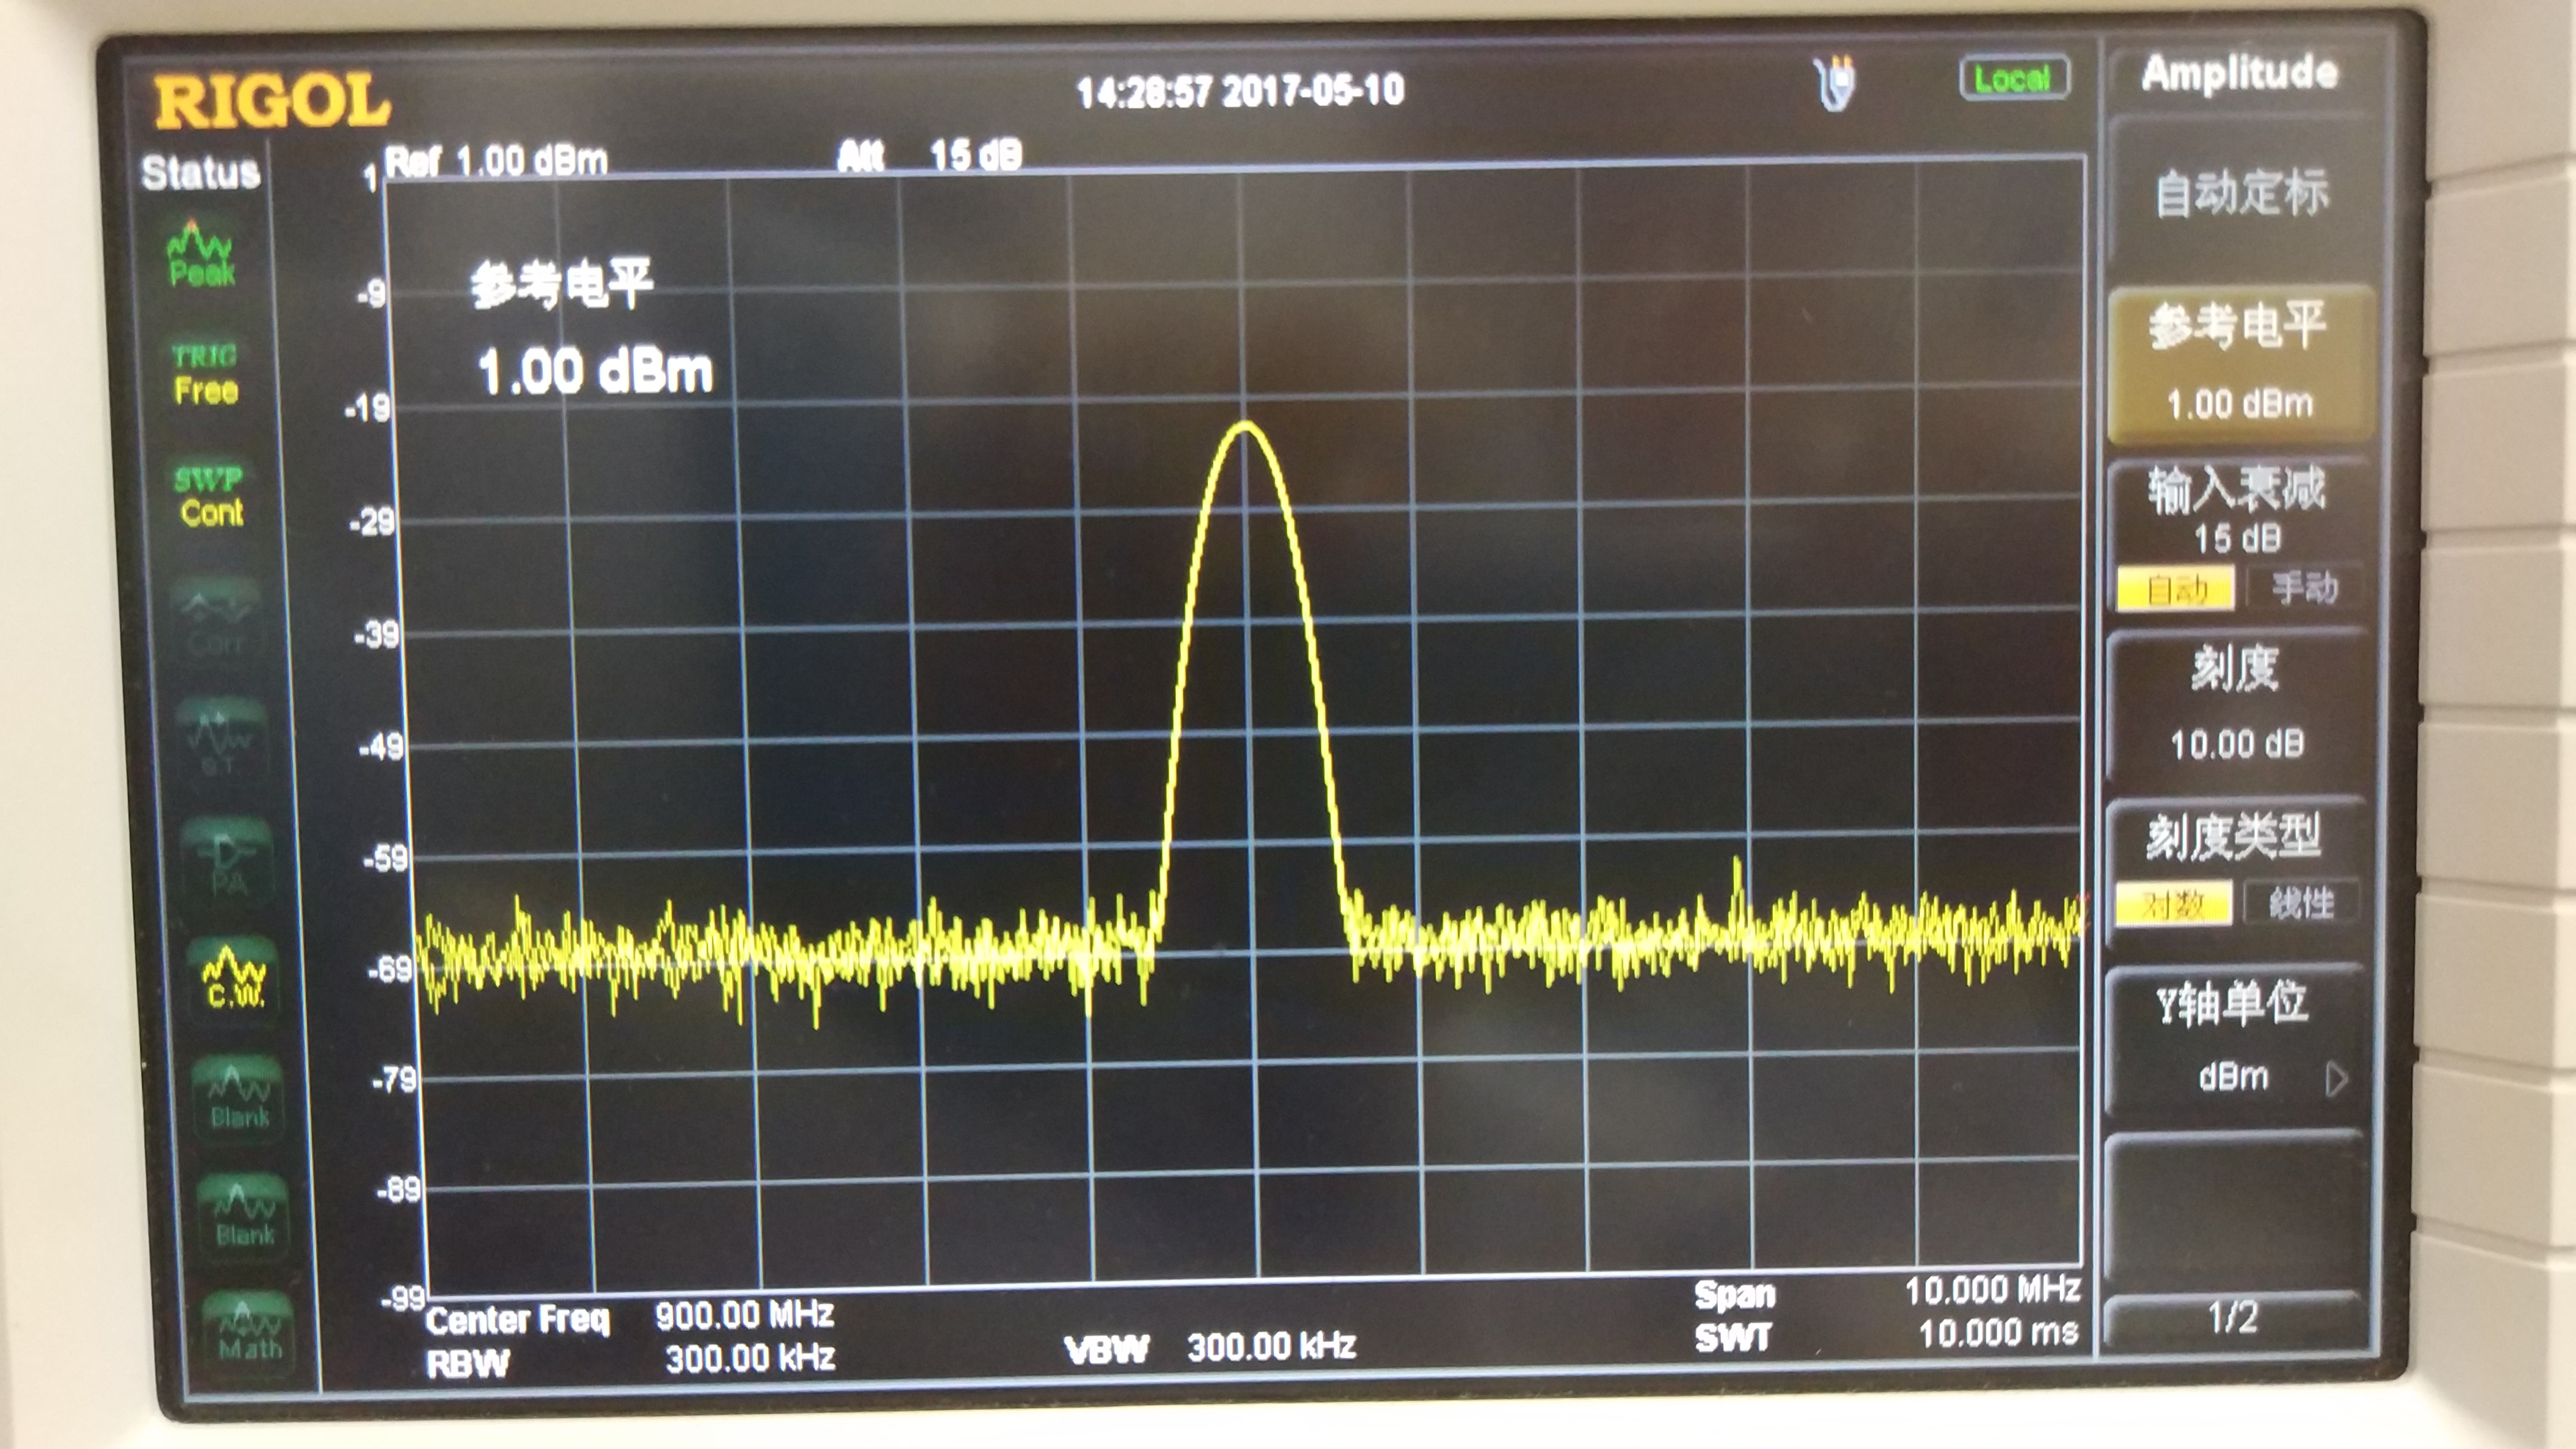
\includegraphics[width=13cm]{figures/uhd_siggen.jpg}
				\caption{uhd\_siggen}
				\label{fig:uhd_siggen}
			\end{figure}
			\par 或者执行
			\begin{lstlisting}[ language = sh ]
uhd_siggen_gui -f 900000000
			\end{lstlisting}
			\par 来运行一个如图\ref{fig:uhd_siggen_gui}的基于GNU Radio的GUI界面。
			\begin{figure}[htp]
				\centering
				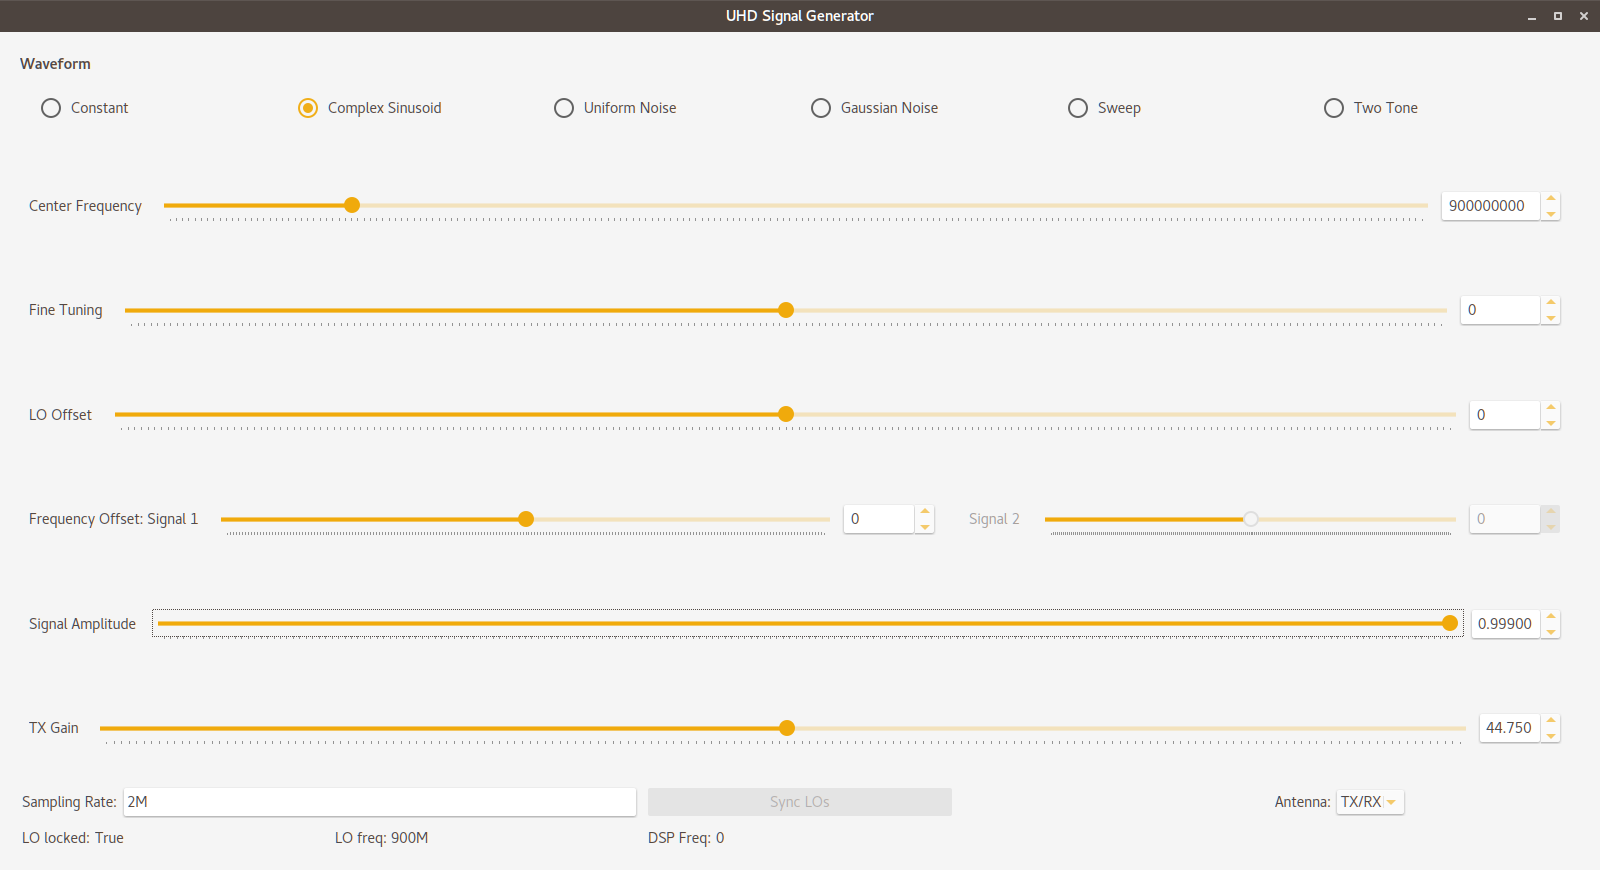
\includegraphics[width=13cm]{figures/uhd_siggen_gui.png}
				\caption{uhd\_siggen\_gui}
				\label{fig:uhd_siggen_gui}
			\end{figure}
	\section{gqrx}
		\subsection{简介}
			\par gqrx是由GNU Radio和Qt图形工具包提供支持的开源软件定义无线电接收器(SDR),用来通过USRP接收无线电信号,可以直接接收FM广播,并提供直观的瀑布图,可以作为没有频谱仪情况下的替代品。
			\par gqrx支持许多SDR硬件,包括Airspy,Funcube Dongles,rtl-sdr,HackRF和USRP设备,gqrx是免费软件,根据GNU通用公共许可证许可,允许任何人修复和修改它以供使用。
			\begin{figure}[htbp]
				\centering
				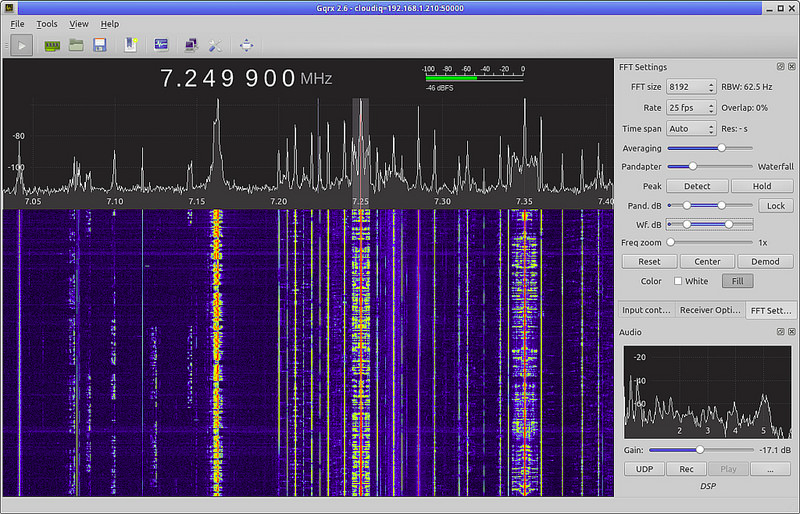
\includegraphics[width=13cm]{figures/gqrx.png}
				\caption{gqrx运行截图}
				\label{fig:gqrx运行截图}
			\end{figure}
			\par gqrx的源码已托管于GitHub(\href{https://github.com/csete/gqrx}{https://github.com/csete/gqrx})。
	\section{git}
		\subsection{简介}
			\par git是用于Linux内核开发的版本控制工具。与CVS、Subversion一类的集中式版本控制工具不同,它采用了分布式版本库的作法,不需要服务器端软件,就可以运作版本控制,使得源代码的发布和交流极其方便。git的速度很快,这对于诸如Linux内核这样的大项目来说自然很重要。git最为出色的是它的合并追踪(merge tracing)能力\ucite{ wiki:Git}。
			\par GNU Radio使用git进行版本控制,在进行源码查看编辑的时候使用git能大大提高开发效率,在此简要介绍其使用方法。
			\par git的一个仓库由三个区组成:工作区,暂存区,版本库。我们平常编写程序的叫做工作区,在工作区中编写程序,修复bug,然后将修改后的文件通过\lstinline[language=sh]{git add -p <file>}	命令添加到暂存区,检查暂存区没有错误以后通过\lstinline[language=sh]{git commit -m "some comments"}命令将修改提交至版本库,如果存在远程仓库还需要执行\lstinline[language=sh]{git push}命令来将修改提交至远程仓库。
			\par 以上是一个正常的提交流程,我们可以通过\lstinline[language=sh]{git log}来查看所有的\lstinline[language=sh]{commit},并通过\lstinline[language=sh]{git reset --hard <your commit flag>}来回退至相应的版本。
			\par 一个好的习惯是在添加新功能或者修复某一个bug时执行\lstinline[language=sh]{git checkout -b fix}创建一个名为\lstinline[language=sh]{fix}的分支,在该分支中修改bug,修改完成并测试通过以后\lstinline[language=sh]{git commit -m "some comments"}将修改提交至本地仓库,再执行\lstinline[language=sh]{git checkout master}并执行\lstinline[language=sh]{git merge fix}来将修改合并至主分支,这样可以在不影响主分支的情况进行bug的修复和新功能的添加。在GitHub上可能还需要执行pull request来将修改提交至源仓库。
			\par git的源码已托管于GitHub(\href{https://github.com/git/git}{https://github.com/git/git})。
		\subsection{常用命令}
			\par $\bullet$ \lstinline[language=sh]{git config --global user.name "Your name"}
			\par 使用仓库之前得先告诉git你是谁,谁提交了接下来的修改。
			\par $\bullet$ \lstinline[language=sh]{git config --global user.email "email@example.com"}
			\par git是外国人开发的,较为正式的联系方式是电子邮件。
			\par $\bullet$ \lstinline[language=sh]{git add -p <file>}
			\par 将文件和修改提交至暂存区,可以使用\lstinline[language=sh]{git add .}命令将所有文件提交至暂存区。
			\par $\bullet$ \lstinline[language=sh]{git commit -m "some comments"}
			\par 将文件和修改提交至本地仓库,并添加一些批注。
			\par $\bullet$ \lstinline[language=sh]{git status}
			\par 显示仓库当前状态。
			\par $\bullet$ \lstinline[language=sh]{}git log
			\par 显示提交日志,可以通过添加\lstinline[language=sh]{--pretty=oneline}参数来格式化输出信息。
			\par $\bullet$ \lstinline[language=sh]{git reset --hard 130f101}
			\par 版本回退,最后的为\lstinline[language=sh]{git log}中的唯一标识,也可以使用\lstinline[language=sh]{HEAD}来撤销更改,回退到当前版本。
			\par $\bullet$ \lstinline[language=sh]{git checkout -- <file>}
			\par 丢弃工作区的修改,回到最近一次的\lstinline[language=sh]{commit}或者\lstinline[language=sh]{add}的状态,该命令可以在\lstinline[language=sh]{git status}中提示。
			\par $\bullet$ \lstinline[language=sh]{git push origin master}
			\par 将修改提交至远程仓库,可以添加多个远程仓库,可以指定分支。
			\par $\bullet$ \lstinline[language=sh]{git diff}
			\par 显示文件于版本库的差异。
			\par $\bullet$ \lstinline[language=sh]{git fetch}
			\par 获取远程仓库的最新版本。
			\par $\bullet$ \lstinline[language=sh]{git pull}
			\par 获取远程仓库的最新版本,并与本地仓库合并。
			\par $\bullet$ \lstinline[language=sh]{git branch dev}
			\par 创建分支。
			\par $\bullet$ \lstinline[language=sh]{git checkout dev}
			\par 切换至dev分支,可以使用\lstinline[language=sh]{git checkout -b dev}来创建并切换至dev分支。
			\par $\bullet$ \lstinline[language=sh]{git merge dev}
			\par 合并指定分支至当前分支。
			\par 在众多教程中,廖雪峰的官方网站(\href{http://www.liaoxuefeng.com/}{http://www.liaoxuefeng.com/})很适合初学者,深入浅出的讲解了使用git过程中常用的许多命令。
			% \subsection{版本控制}
		\subsection{GitHub}
			\par GitHub是一个通过Git进行版本控制的软件源代码托管服务,由GitHub公司(曾称Logical Awesome)的开发者Chris Wanstrath、PJ Hyett和Tom Preston-Werner使用Ruby on Rails编写而成。GitHub同时提供付费账户和免费账户,这两种账户都可以创建公开的代码仓库,但是付费账户还可以创建私有的代码仓库。根据在2009年的Git用户调查,GitHub是最流行的Git访问站点。除了允许个人和组织创建和访问保管中的代码以外,它也提供了一些方便社会化共同软件开发的功能,即一般人口中的社区功能,包括允许用户追踪其他用户、组织、软件库的动态,对软件代码的改动和bug提出评论等\ucite{ wiki:GitHub}。
			\par GitHub的使用与git并无太多区别。
			\par 本设计使用的众多开源库、软件均已托管于GitHub。
	\section{Docker}
		\subsection{简介}
			\par Docker是一个开放源代码软件项目,让应用程序布署在软件容器下的工作可以自动化进行,借此在Linux操作系统上,提供一个额外的软件抽象层,以及操作系统层虚拟化的自动管理机制。Docker利用Linux核心中的资源分脱机制,例如cgroups,以及Linux核心名字空间(name space),来创建独立的软件容器(containers)。这可以在单一Linux实体下运作,避免引导一个虚拟机造成的额外负担。Linux核心对名字空间的支持完全隔离了工作环境中应用程序的视野,包括进程树、网络、用户ID与挂载文件系统,而核心的cgroup提供资源隔离,包括CPU、存储器、block I/O与网络。从0.9版本起,Dockers在使用抽象虚拟是经由libvirt的 LXC与systemd - nspawn提供界面的基础上,开始包括libcontainer库做为以自己的方式开始直接使用由Linux核心提供的虚拟化的设施\ucite{ wiki:Docker}。
			\par 在构建应用时,如果在实机上进行运行测试,很容易因为依赖的问题导致应用无法正常运行,严重时会造成系统的崩溃。Docker提供了一个虚拟的环境来构建自己的应用,同时也能够与git进行版本控制与回滚,在Docker中构建应用也能更快的部署应用。需要大规模部署应用时只需要从仓库中拉取自己需要的环境以及版本,进行少量的配置即可运行。
			\par 本设计由于时间问题并未采用Docker来管理系统镜像版本,在修改系统环境的过程中走了不少弯路,后续开发者可以一开始就在Docker的环境下开发软件,或者在安装Ubuntu时使用LVM,创建快照省去因为系统环境配置出错而频繁的重装系统,保证一个相对纯净的开发环境,同时其他开发者可以直接拉取该镜像以进行二次开发。
			% \subsection{构建容器}
			% TODO: 构建容器
	\section{GNU Radio}
		\label{sec:gnuradio}
		\subsection{简介}
			\par GNU Radio 是免费开源的软件开发工具套件。它提供构建软件无线电所需的信号运行和处理的模块,用它可以在唾手可得的低成本的外部射频(RF)硬件和通用微处理器上、或无硬件的模拟环境中实现软件定义无线电。这套套件广泛用于业余爱好者,学术机构和商业机构用来研究和构建无线通信系统。
			\par GNU Radio 可以进行各类信号处理。可以使用它编写应用程序从数据流中获取数据或将数据传输到数据流中,然后使用硬件将其发射出去。GNU Radio 具有滤波器、通道编码、同步单元、均衡单元(equalizer)、解调器、声音合成机(vocoder)、解码器(decoder)、等很多单元(使用 GNU Radio 术语,这些被称作功能块 - blocks),这些单元也都是无线电系统中的常见部件单元。更重要的是,它还具有连接这些功能模块的方法及管理在这些功能块间传输数据的策略。
			\par GNU Radio 的应用主要是用 Python 编程语言来编写的。但是其核心信号处理模块是 C++ 在带浮点运算的微处理器上构建的。因此,开发者能够简单快速的构建一个实时、高容量的无线通信系统\ucite{what_is_gnuradio}。
			\par GNU Radio的使用方法类似于Matlab中的SimuLink,通过拖动框图来构建通信系统,并能够生成一个Python文件,如果使用No Gui就能够生成命令行下可以直接运行的程序。因为其有友好的GUI界面,此处不再赘述使用方法。
		\subsection{安装}
			\par GNU Radio安裝有两种方式:源码编译和通过包管理程序安装,包管理程序安装方式包括两种:apt-get和PyBOMBS。
			\par\noindent $\bullet$ 源码编译
			\par GNU Radio需要的依赖参看\href{https://gnuradio.org/doc/doxygen/build\_guide.html}{https://gnuradio.org/doc/doxygen/build\_guide.html},所有依赖均可以通过apt-get的方式进行安装,这种方式可以保证软件版本较新,但是安装时间较长,编译时间可能长达数小时,所以大多数情况下采用包管理程序安装。
			\par\noindent $\bullet$ 包管理安装
			\par\noindent \qquad$\circ$ apt-get
			\par Ubuntu:
			\par Ubuntu 16.04的源中提供的版本为3.7.9,需要手动编译gr-dvbt(参见\ref{sec:gr-dvbt_compile}节),Ubuntu 17.04中的源已经更新至3.7.10,已经内置了gr-dvbt,不需要再手动编译了,安装GNU Radio时推荐使用新立得包管理软件(Synaptic)。
			\par 树莓派:
			\par 树莓派默认的软件源为jessie,提供的最新版本为3.7.5,需要手动编译gr-dvbt(参见\ref{sec:gr-dvbt_compile}节)。如果需要安装3.7.10版本,需要切换软件源为stretch源(stretch为testing源),修改\lstinline[language=sh]{/etc/apt/source.list}文件,将其中的jessie修改为stretch。
			\begin{lstlisting}
deb http://mirrors.ustc.edu.cn/raspbian/raspbian/ stretch main non-free contrib 
deb-src http://mirrors.ustc.edu.cn/raspbian/raspbian/ stretch main non-free contrib
			\end{lstlisting}
			\par 修改完成后执行
			\begin{lstlisting}
sudo apt update
sudo apt install gnuradio-dev
			\end{lstlisting}
			\par 安装完成之后使用python测试,gnuradio需要Python 2环境,在Python 3环境下无法运行。
			\begin{lstlisting}[ language= sh ]
Python 2.7.13 (default, Jan 19 2017, 14:48:08)
[GCC 6.3.0 20170118] on linux2
Type "help", "copyright", "credits" or "license" for more information.
>>> import gnuradio
>>>
			\end{lstlisting}
			\par 如果没有出现\lstinline[language=sh]{no module named gnuradio}则表示安装成功。
			\par\noindent \qquad$\circ$ PyBOMBS
			\par 安装PyBOMBS
			\begin{lstlisting}[ language= sh ]
sudo pip install PyBOMBS
			\end{lstlisting}
			\par 或者
			\begin{lstlisting}[ language= sh ]
git clone https://github.com/gnuradio/pybombs.git
cd pybombs
sudo python setup.py install
			\end{lstlisting}
			\par 添加PyBOMBS源
			\begin{lstlisting}[ language= sh ]
pybombs recipes add gr-recipes git+https://github.com/gnuradio/gr-recipes.git  
pybombs recipes add gr-etcetera git+https://github.com/gnuradio/gr-etcetera.git
			\end{lstlisting}
			\par 配置安装参数
			\begin{lstlisting}[ language= sh ]
pybombs prefix init ~/prefix/default/
			\end{lstlisting}
			\par 安装GNU Radio
			\begin{lstlisting}[ language= sh ]
pybombs install gnuradio
			\end{lstlisting}
			\par 运行GNU Radio Companion
			\begin{lstlisting}[ language= sh ]
pybombs run gnuradio-companion
			\end{lstlisting}
		\subsection{gr-dvbt编译}
			\label{sec:gr-dvbt_compile}
			\par gr-dvbt源码已托管于GitHub(\href{https://github.com/BogdanDIA/gr-dvbt}{https://github.com/BogdanDIA/gr-dvbt})。
			\par 3.7.9及以下版本的GNU Radio需要从源码编译,首先安装相关依赖,一般情况下需要以下依赖:
			\begin{lstlisting}[ language= sh ]
sudo apt install log4cpp libboost-all-dev swig git cmake
			\end{lstlisting}
			\par 编译并运行
			\begin{lstlisting}[ language= sh ]
git clone https://github.com/BogdanDIA/gr-dvbt.git
cd gr-dvbt
mkdir build
cd build
cmake ../
make && sudo make install
			\end{lstlisting}
			\par 如果是第一次安装还需要链接动态库
			\begin{lstlisting}[ language= sh ]
sudo ldconfig
			\end{lstlisting}
			\par\noindent $\bullet$ 树莓派
			\par 由于gr-dvbt使用了维特比解码,并且在其中调用了\lstinline{xmmintrin.h},使用x86平台下的汇编来进行计算加速,导致无法在树莓派平台上成功编译。但是,维特比解码仅在接收端使用,所以可以注释其中与维特比有关的代码段来成功编译,并运行发射端程序。
			\par \lstinline{/lib/CMakeLists.txt}中注释以下行
			\begin{lstlisting}
......
# viterbi_decoder_impl.cc
# d_viterbi.c
......
# ${CMAKE_CURRENT_SOURCE_DIR}/qa_viterbi_decoder.cc

			\end{lstlisting}
			\par 去掉其中的\lstinline{-msse2}参数
			\begin{lstlisting}
set(CMAKE_CXX_FLAGS "${CMAKE_CXX_FLAGS} -Wall -O3 -funroll-loops -msse2")
set(CMAKE_CXX_FLAGS "${CMAKE_CXX_FLAGS} -Wall -O3 -funroll-loops -msse2")
			\end{lstlisting}
			\par \lstinline{/python/CMakeLists.txt}中注释以下行
			\begin{lstlisting}
GR_ADD_TEST(qa_viterbi_decoder ${PYTHON_EXECUTABLE} ${CMAKE_CURRENT_SOURCE_DIR}/qa_viterbi_decoder.py)
			\end{lstlisting}
			\par \lstinline{/swig/dvbt_swig.i}中注释以下行
			\begin{lstlisting}
......
// #include "dvbt/viterbi_decoder.h"
......
// %include "dvbt/viterbi_decoder.h"
......
// GR_SWIG_BLOCK_MAGIC2(dvbt, viterbi_decoder);
			\end{lstlisting}
			\par 执行
			\begin{lstlisting}[ language= sh ]
git clone https://github.com/BogdanDIA/gr-dvbt.git
cd gr-dvbt
mkdir build
cd build
cmake ../
make && sudo make install
sudo ldconfig
			\end{lstlisting}
			\par 之后便可以通过GNU Radio调用gr-dvbt的相关框图。